\chapter{Introducción}
Los avances en teoría de lenguajes de programación han sido durante la historia de la informática una pieza imprescindible sobre la que se han sustentado las aplicaciones prácticas de la ciencia de la computación. Nadie soñaría con tener sistemas funcionales con el nivel de complejidad actual si solo contásemos con herramientas de bajo nivel como la modificación manual de binarios o el lenguaje ensamblador. Las diferentes mejoras que se han ido sucediendo nos han dado herramientas, como la programación funcional y la orientación a objetos, con las que contrarrestar el incremento exponencial en complejidad que surge de tener estados globales. Mediante los sistemas de tipos seguros podemos garantizar que un programa no terminará de forma inesperada y encontrar fallos en el software sin tener que ejecutarlo con todas sus posibles variantes. La gestión automática de la memoria, las funciones de primer orden, o construcciones tan básicas como los condicionales y los bucles han hecho la programación una tarea mucho más cómoda y accesible a un conjunto mayor de la población. El estudio de las técnicas para diseñar e implementar lenguajes han hecho que los compiladores y los intérpretes dejen de ser de las piezas de software más difíciles de realizar, como lo fueron en su época, eliminando a su vez restricciones sobre los tipos de gramática que se pueden manejar. Esto a dado como resultado una gran cantidad de lenguajes específicos para dominios concretos que han hecho más fácil la vida de muchas personas, tales como \textit{SQL}, \textit{Prolog}, \textit{Mathlab}, \textit{Mathematica}, \textit{R} o \textit{Bash}.\\

Podría pensarse que las grandes contribuciones a la teoría de lenguajes de programación ya han sido realizadas, y que los lenguajes que tenemos, salvo algunos retoques, son lo suficientemente buenos. Sin embargo, en los últimos años estamos atendiendo a un surgimiento de nuevos lenguajes y técnicas que traen ideas frescas a la mesa. Por ejemplo \textit{Idris} y los tipos dependientes, \textit{Elm} y la unión e intersección de tipos, \textit{Racket} y su ecosistema para la ``programación orientada a lenguajes'', \textit{Cristal} utilizando elementos que hasta ahora han sido propios de los lenguajes interpretados y combinándolos en un lenguaje compilado de alto rendimiento, o \textit{Rust}, que ha revolucionado el mundo de la programación de sistemas con su particular forma de gestionar la memoria, que evita errores propios de lenguajes con manejo de memoria manual así como problemas de condiciones de carrera en programas concurrentes.\\

En nuestra opinión una de las ramas en la que se están produciendo avances más interesantes es la de los sistemas de tipos, y es precisamente en este campo en el que enfocaremos el TFG. Desde la inspiración que supone la teoría de tipos, pasando por la teoría que hay detrás de estos sistemas, para terminar diseñando e implementando uno propio para un lenguaje especializado en inteligencia artificial, un nicho que creo aún no ha sido rellenado de forma satisfactoria por ningún otro lenguaje.\\

Las principales referencias para este trabajo serán \textit{Homotopy Type Theory: Univalent Foundations of Mathematics} \cite{hottbook} para la parte de teoría de tipos ,\textit{Types and Programming Languages} \cite{TPL} para los sitemas de cálculo y de tipos y \textit{Compilers: Principles, Techniques, and Tools} \cite{dragoonBook} para la implementación.\\

\section{Objetivos del TFG}
Los principales objetivos del TFG son los siguientes:\\

\begin{itemize}
	\item Servir como introducción a la teoría de lenguajes de programación\\
	
	El objetivo principal de este TFG es la de estudiar y explicar los fundamentos de la teoría de lenguajes de programación, cubriendo sistemas de cálculo, sistemas de tipos e implementación de procesadores de lenguajes. Esta tarea se lleva a cabo a lo largo de todo el trabajo, pero tal vez la parte más representativa sea el capítulo \ref{sect:sistemas_de_calculo}.\\
	
	\item Estudiar la relación entre la teoría de tipos y los sistemas de tipos\\
	
	Se presentará una introducción a la teoría de tipos, desde sus motivaciones matemáticas y resultados teóricos hasta su influencia en los sistemas de tipos usados en la actualidad.
	Este estudio se realiza mayoritariamente en el capítulo \ref{sect:tt}.\\
	
	\item Proponer un lenguaje especializado en inteligencia artificial\\
	
	Se estudiarán cuales son los elementos que pueden aumentar la utilidad de un lenguaje en este campo y, una vez determinados, se tendrán en cuenta en el diseño de un nuevo lenguaje, utilizando para ello las técnicas ya estudiadas. La fase de estudio se puede encontrar en el capítulo \ref{sect:ap_ia} y la de diseño en el \ref{sect:form_tail}.\\
	
	\item Implementar un compilador para dicho lenguaje\\
	
	Se programará un software capaz de ejecutar programas escritos en este lenguaje, incluyendo las fases de análisis sintáctico, análisis semántico y generación de código. Desgraciadamente este objetivo no ha podido ser completado en su totalidad, ya que han surgido dificultades en la generación de código. Esta parte se expone en el capítulo \ref{sect:impl}.\\
\end{itemize}

\section{Principales aportaciones del TFG}
Las principales aportaciones del TFG son las siguientes:\\

\begin{itemize}
	\item Recopilación de técnicas para el análisis de lenguajes\\
	
	Se recogen y explican diversas técnicas ampliamente utilizadas en el diseño y análisis teórico de los lenguajes de programación.\\
	
	\item Investigación sobre sistemas de tipos novedosos\\
	
	Se estudia e implementa el sistema de unión e intersección de tipos graduales, un sistema de tipos avanzado y de desarrollo reciente que todavía no se encuentra disponible en ningún lenguaje mayoritario.\\
	
	\item Propuesta de un lenguaje orientado a la inteligencia artificial\\
	
	Se aplican las técnicas anteriores en el diseño de un lenguaje que, a nuestro parecer, es útil en el campo de la inteligencia artificial.\\
	
	\item Implementación de un compilador para dicho lenguaje\\
	
	Se ofrece un software capaz de ejecutar programas escritos en el lenguaje diseñado.\\
\end{itemize}


\section{Temporización}

Inicialmente la planificación del proyecto seguía el siguiente esquema. Durante el verano se comenzaría con la lectura de la bibliografía básica, para obtener una visión general de la materia y adquirir los conocimientos necesarios para comenzar con el TFG. Acto seguido se profundizaría en conceptos más avanzados para, haciendo uso de ellos, empezar a diseñar el lenguaje. La implementación se dejaría para la segunda mitad del año. Un diagrama de este plan se puede ver en la figura \ref{fig:gantt1}.\\

Sin embargo, el plan inicial no contaba con la exigencia de tiempo que demandaría el curso académico, en particular en los periodos de exámenes, que produjo un descenso notable en la productividad. Como consecuencia fue necesario continuar el desarrollo durante los meses de julio y agosto. En la figura \ref{fig:gantt2} se muestra una aproximación de la distribución real del trabajo.\\

Como se observa, durante el verano se cumplieron los objetivos. Esto cambió en diciembre, debido a las entregas de trabajos y exámenes parciales propios de la época no se pudieron llevar a cabo las demostraciones sobre las propiedades del lenguaje, que se trasladaron al mes de julio. 
Aún así se aprovechó el periodo vacacional para implementar el analizador sintáctico del lenguaje. El avance se frenó en seco durante el periodo de exámenes de febrero, haciéndose algunas aportaciones a la memoria durante los meses de marzo y abril.\\

\begin{landscape}
	\begin{figure}[h]
		\begin{center}
			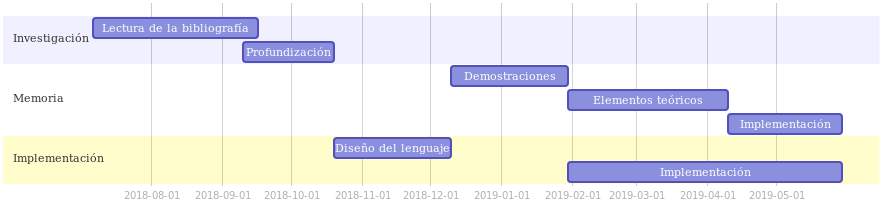
\includegraphics[width=1.6\textwidth]{imagenes/gantt1.png}
			\caption{Diagrama de Gantt del plan inicial}
			\label{fig:gantt1}
			\bigskip
			\bigskip
			\bigskip
			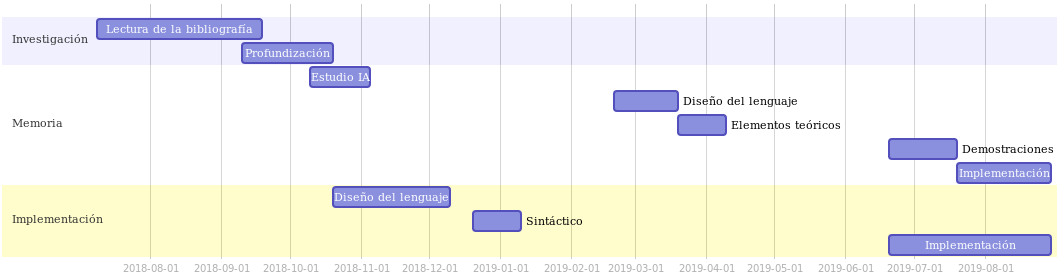
\includegraphics[width=1.6\textwidth]{imagenes/gantt2.png}
			\caption{Diagrama aproximado del trabajo real}
			\label{fig:gantt2}
		\end{center}
	\end{figure}
\end{landscape}